%\begin{sidewaysfigure}
%  \begin{center}
%  \includegraphics[width=0.8\textheight]{lhcb-detector-cross-section}
%  \caption[Cross-section view of \LHCb, cut in the non-bending $y$--$z$ plane]%
%    {Cross-section view of \LHCb, cut in the non-bending $y$--$z$ plane.}
%  \label{fig:LHCbCrossSection}
%  \end{center}
%\end{sidewaysfigure}



\chapter{Measurement of the $\nu_\mu$ charged current inclusive cross-section on Pb}
\label{chap:CrossSectionMeasurement}
This chapter presents the measurement of the $\nu_\mu$ CC inclusive cross-section on Pb using the ND280 ECals.  This chapter details the measurement method, the samples used in the measurement, the assessment of the systematic uncertainties, validation of the measurement method and finally the measurement itself.

\section{Measurement method}
\label{sec:MeasurementMethod}
The chosen method~\cite{PhysRevD.78.032003, PhysRevD.83.012005} fits a prediction to measured data using multiple data samples.  The core of the analysis method is a $\chi^2$ fit which tries to minimise the difference between the prediction and the data.  The $\chi^2$ is defined as 
\begin{equation}
  \chi^2 = \Delta \vec{N}^{\textrm{T}} \left(\underline{\underline{V}}^{\textrm{syst}} + \underline{\underline{V}}^{\textrm{stat}} \right)^{-1} \Delta \vec{N},
  \label{eqn:Chi2Def}
\end{equation}
where $\underline{\underline{V^{\textrm{syst}}}}$ and $\underline{\underline{V^{\textrm{stat}}}}$ are the systematic and statistical covariance matrices for the sample and $\Delta\vec{N}$ contains the difference between the data and the prediction for each sample.  If the number of samples used is $M$, $\Delta\vec{N}$ is defined as 
\begin{equation}
  \Delta\vec{N} = 
  \begin{pmatrix}
    N^{\textrm{data}}_1 - N^{\textrm{pred}}_1 \\
    \vdots \\
    N^{\textrm{data}}_M - N^{\textrm{pred}}_M
  \end{pmatrix}.
  \label{eqn:VecNDef}
\end{equation}
For sample $j$ of the sample set $M$, $N^{\textrm{data}}_j$ and $N^{\textrm{pred}}_j$ are the number of measured data events and number of predicted events.  The extractable information from the fit is located in $N^{\textrm{pred}}_j$ which can be subdivided into a set of templates, each of which are assigned a normalisation parameter, namely
\begin{equation}
  N^{\textrm{pred}}_j = \sum_j R_{i}n_{ij},
  \label{eqn:NPredDef}
\end{equation}
where $n_{ij}$ is the number of events in template $i$ of sample $j$ and $R_{i}$ is the normalisation assigned to that template.  The normalisation parameters are free to float in the fit and so it  is in the normisation parameters that the desired physical information is located.
\section{Input samples to the fit}
\label{sec:InputSamples}
The DS ECal provides the main signal sample which will be used to extract the cross-section.  As shown in table~\ref{table:FinalEffPur}, the selected sample in the DS ECal has the highest purity and efficiency in the whole selection making the sample the natural choice to extract the cross-section.
\newline
\newline
The method outlined above allows for the simultaneous constraint of a physical parameter and the background contamination of a set of input samples.  The method works particularly well when the input samples do not share the same sensitivity to a particular background type.  For example, in ND280, each ECal module is exposed to a different beam intensity and energy spectrum and so is exposed to a unique amount of beam induced background.  Each ECal module can be thought of as a separate input sample which fits well with the method outlined above.  So, while the DS ECal will provide the target in which the cross-section will be extracted, the barrel ECals are to also be included in the fit as a background constraint.  To further allow the barrel ECals to achieve this, an additional sample of barrel ECal events are to be included.  This additional sample set, called the 'reverse' sample set,  comes from the same data set as the selected sample described in chapter~\ref{chap:NeutrinoInteractionSelection}.  However, the events in the reverse sample set are events which pass the fiducial volume cuts but fail any other cut.  An example of a selected sample compared with a reverse sample is shown in Fig.~\ref{fig:NuEnergyReactionCodeBottomLeft}.  There are clear differences in the shape of the energy spectrum between Fig.~\ref{fig:NuEnergyReactionCodeBottomLeftSignal} and Fig.~\ref{fig:NuEnergyReactionCodeBottomLeftReverse} which suggests that the selection is biased towards lower energy neutrino interactions, despite the flat efficiency curves shown in Fig.~\ref{fig:EffPurSummedTopologiesBarrel}. The apparent bias is actually an effect of higher energy interactions creating a surplus of reconstructed events, most of which are cut away by the selection.  The shape of the true neutrino energy spectrum (see Fig.~\ref{fig:NSignalEventsTruthNeutrinoEnergy} for an example) is actually more like the selected sample shown in Fig.~\ref{fig:NuEnergyReactionCodeBottomLeftSignal}.
\begin{figure}%
  \centering
  \subfloat[Selected sample.]{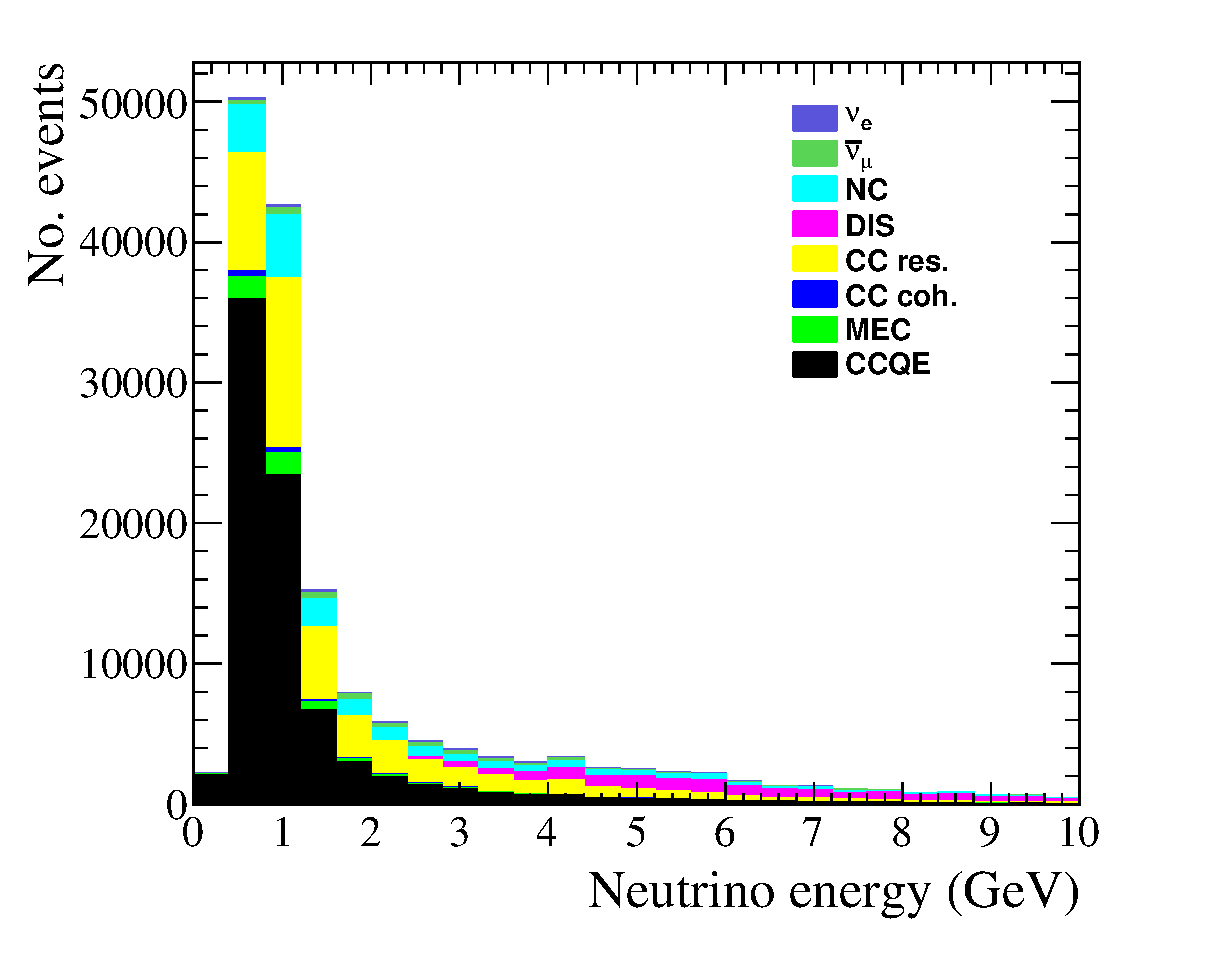
\includegraphics[width=8cm]{images/measurement/samples/NuEnergy_ReactionCode_BottomLeft_Signal.eps} \label{fig:NuEnergyReactionCodeBottomLeftSignal}}
  \subfloat[Reverse sample.]{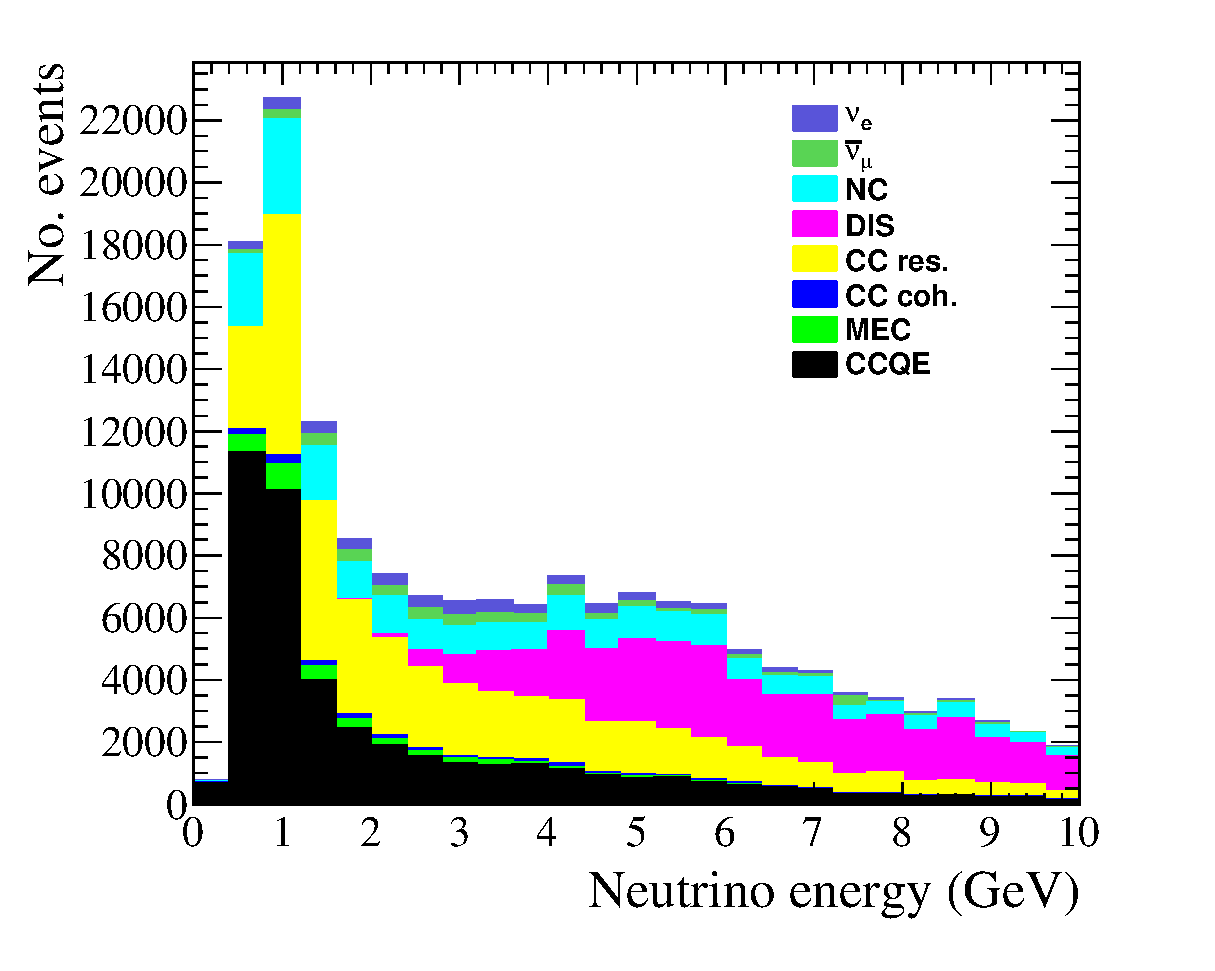
\includegraphics[width=8cm]{images/measurement/samples/NuEnergy_ReactionCode_BottomLeft_Reverse.eps} \label{fig:NuEnergyReactionCodeBottomLeftReverse}}
  \caption{The neutrino energy of events seen in the bottom-left ECal module broken down by the neutrino interaction mode.}
  \label{fig:NuEnergyReactionCodeBottomLeft}
\end{figure}
\newline
\newline
As described in chapter~\ref{chap:NeutrinoInteractionSelection}, the developed selection does not distinguish between lead and carbon interactions, partly because such events are indistinguishable from one another.  It is however desirable to separate the two catagories out as the presented measurement purely involves lead.  As the ECal is not capable of separating the events by itself, an additional constraint is needed.  So, a sample of CC interactions on carbon occurring in the FGD are also included, which are taken from the official ND280 oscillation input analysis [INSERT TECHNOET REFERENCE!!!!!].
\newline
\newline
To summarise, there are many inputs samples to the measurement.  Specifically, there are 12 barrel ECal samples (6 selected and 6 reverse), the DS ECal sample and the FGD sample which totals to 12 input samples.

\section{The ECal rate fit}
\label{sec:ECalRateFit}
Now that the general method and the input samples have been introduced, the fit used by the analysis can be introduced.  The fit itself is a data-driven constraint of the event rate in each ECal module where the Monte Carlo prediction is separated into templates whose normalisation is allowed to vary.  The machinery outlined in section~\ref{sec:MeasurementMethod} almost completely decribes what is required to understand the fit, however two specific definitions are needed.  The first is that there are 12 input samples to the fit.  The second is the definition of $N^{\textrm{pred}}_i$.  To constrain the lead event rate, three Monte Carlo templates are needed: a lead template which contains any reconstructed event associated with a $\nu_\mu$ CC interaction on lead, a carbon template which contains any reconstructed event associated with a $\nu\mu$ CC interaction on carbon and an 'other' template which contains any reconstructed event which does not fall into the above two catagories.  $N^{\textrm{pred}}_i$ is then defined as 
\begin{equation}
  N^{\textrm{pred}}_i = R^{\textrm{Pb}}n^{\textrm{Pb}}_i + R^{\textrm{C}}n^{\textrm{C}}_i + R^{\textrm{other}}n^{\textrm{other}}_i,
  \label{eqn:ECalFitPredDef}
\end{equation}
where $n^{\textrm{X}}_i$ is the number of events in template X of sample $i$ and $R^{\textrm{X}}_i$ is the variable normalisation of that template.
\newline
\newline
The rate fit allows $R^{\textrm{Pb}}_i$, $R^{\textrm{C}}_i$ and $R^{\textrm{oth}}_i$ to vary with no prior constraint in an attempt to minimise the $chi^{2}$ as defined in equation~\ref{eqn:Chi2Def}.  Once the minimum has been found, the fitted $R^{\textrm{Pb}}_i$ can then be used to extract the cross-section using the selected events in the DS ECal.  
\newline
\newline
The number of events in each input sample, broken down by the template contribution, is shown in Fig.~\ref{fig:NominalMCTemplates}.  As should be expected, the relative backround contribution varies between each ECal module.
\begin{figure}
  \centering
  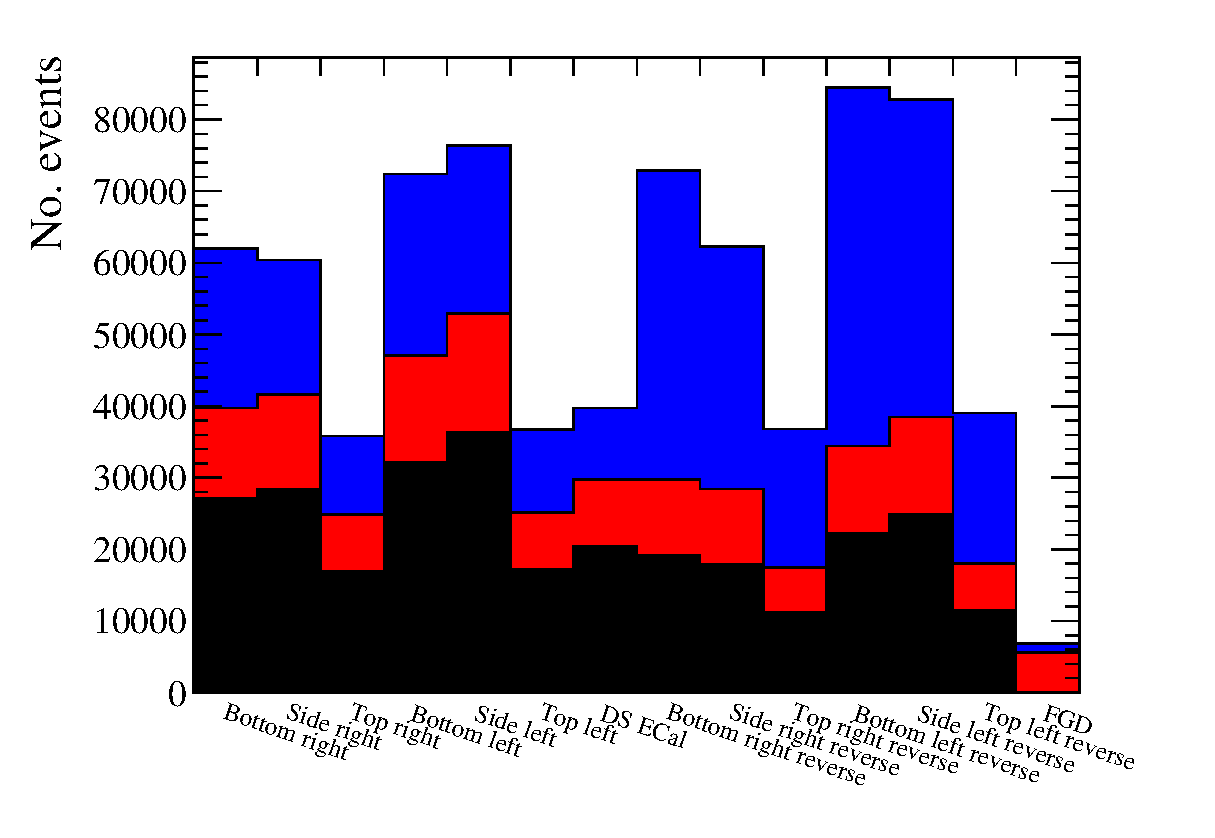
\includegraphics[width=15cm]{images/measurement/rate_fit/MC_Templates_Nominal.eps}
  \caption{The number of events in each input sample separated into the lead (black), carbon (red) and other (blue) templates.}
  \label{fig:NominalMCTemplates}
\end{figure}
\newline
\newline
The underlying fit machinery uses the Minuit2 algorithm provided by the ROOT TFitter framework, chosen primarily because of its ease of use.


\section{Systematic uncertainties}
\label{sec:SystematicUncertainties}

\section{Validation of method}
\label{sec:MethodValidation}
Does it work?

\section{Applying the fit to ND280 data}
\label{sec:ND280DataFit}
Run it


